\documentclass[twoside]{book}

% Packages required by doxygen
\usepackage{fixltx2e}
\usepackage{calc}
\usepackage{doxygen}
\usepackage[export]{adjustbox} % also loads graphicx
\usepackage{graphicx}
\usepackage[utf8]{inputenc}
\usepackage{makeidx}
\usepackage{multicol}
\usepackage{multirow}
\PassOptionsToPackage{warn}{textcomp}
\usepackage{textcomp}
\usepackage[nointegrals]{wasysym}
\usepackage[table]{xcolor}

% Font selection
\usepackage[T1]{fontenc}
\usepackage[scaled=.90]{helvet}
\usepackage{courier}
\usepackage{amssymb}
\usepackage{sectsty}
\renewcommand{\familydefault}{\sfdefault}
\allsectionsfont{%
  \fontseries{bc}\selectfont%
  \color{darkgray}%
}
\renewcommand{\DoxyLabelFont}{%
  \fontseries{bc}\selectfont%
  \color{darkgray}%
}
\newcommand{\+}{\discretionary{\mbox{\scriptsize$\hookleftarrow$}}{}{}}

% Page & text layout
\usepackage{geometry}
\geometry{%
  a4paper,%
  top=2.5cm,%
  bottom=2.5cm,%
  left=2.5cm,%
  right=2.5cm%
}
\tolerance=750
\hfuzz=15pt
\hbadness=750
\setlength{\emergencystretch}{15pt}
\setlength{\parindent}{0cm}
\setlength{\parskip}{3ex plus 2ex minus 2ex}
\makeatletter
\renewcommand{\paragraph}{%
  \@startsection{paragraph}{4}{0ex}{-1.0ex}{1.0ex}{%
    \normalfont\normalsize\bfseries\SS@parafont%
  }%
}
\renewcommand{\subparagraph}{%
  \@startsection{subparagraph}{5}{0ex}{-1.0ex}{1.0ex}{%
    \normalfont\normalsize\bfseries\SS@subparafont%
  }%
}
\makeatother

% Headers & footers
\usepackage{fancyhdr}
\pagestyle{fancyplain}
\fancyhead[LE]{\fancyplain{}{\bfseries\thepage}}
\fancyhead[CE]{\fancyplain{}{}}
\fancyhead[RE]{\fancyplain{}{\bfseries\leftmark}}
\fancyhead[LO]{\fancyplain{}{\bfseries\rightmark}}
\fancyhead[CO]{\fancyplain{}{}}
\fancyhead[RO]{\fancyplain{}{\bfseries\thepage}}
\fancyfoot[LE]{\fancyplain{}{}}
\fancyfoot[CE]{\fancyplain{}{}}
\fancyfoot[RE]{\fancyplain{}{\bfseries\scriptsize Generated by Doxygen }}
\fancyfoot[LO]{\fancyplain{}{\bfseries\scriptsize Generated by Doxygen }}
\fancyfoot[CO]{\fancyplain{}{}}
\fancyfoot[RO]{\fancyplain{}{}}
\renewcommand{\footrulewidth}{0.4pt}
\renewcommand{\chaptermark}[1]{%
  \markboth{#1}{}%
}
\renewcommand{\sectionmark}[1]{%
  \markright{\thesection\ #1}%
}

% Indices & bibliography
\usepackage{natbib}
\usepackage[titles]{tocloft}
\setcounter{tocdepth}{3}
\setcounter{secnumdepth}{5}
\makeindex

% Hyperlinks (required, but should be loaded last)
\usepackage{ifpdf}
\ifpdf
  \usepackage[pdftex,pagebackref=true]{hyperref}
\else
  \usepackage[ps2pdf,pagebackref=true]{hyperref}
\fi
\hypersetup{%
  colorlinks=true,%
  linkcolor=blue,%
  citecolor=blue,%
  unicode%
}

% Custom commands
\newcommand{\clearemptydoublepage}{%
  \newpage{\pagestyle{empty}\cleardoublepage}%
}

\usepackage{caption}
\captionsetup{labelsep=space,justification=centering,font={bf},singlelinecheck=off,skip=4pt,position=top}

%===== C O N T E N T S =====

\begin{document}

% Titlepage & ToC
\hypersetup{pageanchor=false,
             bookmarksnumbered=true,
             pdfencoding=unicode
            }
\pagenumbering{roman}
\begin{titlepage}
\vspace*{7cm}
\begin{center}%
{\Large agv\+\_\+navigation \\[1ex]\large 1 }\\
\vspace*{1cm}
{\large Generated by Doxygen 1.8.11}\\
\end{center}
\end{titlepage}
\clearemptydoublepage
\tableofcontents
\clearemptydoublepage
\pagenumbering{arabic}
\hypersetup{pageanchor=true}

%--- Begin generated contents ---
\chapter{Namespace Index}
\section{Namespace List}
Here is a list of all documented namespaces with brief descriptions\+:\begin{DoxyCompactList}
\item\contentsline{section}{\hyperlink{namespaceturtlebot__rrt}{turtlebot\+\_\+rrt} }{\pageref{namespaceturtlebot__rrt}}{}
\end{DoxyCompactList}

\chapter{Hierarchical Index}
\section{Class Hierarchy}
This inheritance list is sorted roughly, but not completely, alphabetically\+:\begin{DoxyCompactList}
\item \contentsline{section}{Agv}{\pageref{classAgv}}{}
\item Base\+Global\+Planner\begin{DoxyCompactList}
\item \contentsline{section}{turtlebot\+\_\+rrt\+:\+:R\+R\+T\+Planner}{\pageref{classturtlebot__rrt_1_1RRTPlanner}}{}
\end{DoxyCompactList}
\item \contentsline{section}{Explorer}{\pageref{classExplorer}}{}
\item \contentsline{section}{turtlebot\+\_\+rrt\+:\+:Vertex}{\pageref{classturtlebot__rrt_1_1Vertex}}{}
\end{DoxyCompactList}

\chapter{Class Index}
\section{Class List}
Here are the classes, structs, unions and interfaces with brief descriptions\+:\begin{DoxyCompactList}
\item\contentsline{section}{\hyperlink{classAgv}{Agv} \\*\hyperlink{classAgv}{Agv} class }{\pageref{classAgv}}{}
\item\contentsline{section}{\hyperlink{classExplorer}{Explorer} }{\pageref{classExplorer}}{}
\item\contentsline{section}{\hyperlink{classturtlebot__rrt_1_1RRTPlanner}{turtlebot\+\_\+rrt\+::\+R\+R\+T\+Planner} }{\pageref{classturtlebot__rrt_1_1RRTPlanner}}{}
\item\contentsline{section}{\hyperlink{classturtlebot__rrt_1_1Vertex}{turtlebot\+\_\+rrt\+::\+Vertex} }{\pageref{classturtlebot__rrt_1_1Vertex}}{}
\end{DoxyCompactList}

\chapter{File Index}
\section{File List}
Here is a list of all documented files with brief descriptions\+:\begin{DoxyCompactList}
\item\contentsline{section}{/home/bob/catkin\+\_\+ws/src/agv\+\_\+navigation/include/{\bfseries Agv.\+hpp} }{\pageref{Agv_8hpp}}{}
\item\contentsline{section}{/home/bob/catkin\+\_\+ws/src/agv\+\_\+navigation/include/{\bfseries Explorer.\+hpp} }{\pageref{Explorer_8hpp}}{}
\item\contentsline{section}{/home/bob/catkin\+\_\+ws/src/agv\+\_\+navigation/include/turtlebot\+\_\+rrt/{\bfseries turtlebot\+\_\+rrt.\+hpp} }{\pageref{turtlebot__rrt_8hpp}}{}
\item\contentsline{section}{/home/bob/catkin\+\_\+ws/src/agv\+\_\+navigation/include/turtlebot\+\_\+rrt/{\bfseries vertex.\+hpp} }{\pageref{vertex_8hpp}}{}
\item\contentsline{section}{/home/bob/catkin\+\_\+ws/src/agv\+\_\+navigation/src/\hyperlink{vertex_8cpp}{vertex.\+cpp} }{\pageref{vertex_8cpp}}{}
\end{DoxyCompactList}

\chapter{Namespace Documentation}
\hypertarget{namespaceturtlebot__rrt}{}\section{turtlebot\+\_\+rrt Namespace Reference}
\label{namespaceturtlebot__rrt}\index{turtlebot\+\_\+rrt@{turtlebot\+\_\+rrt}}
\subsection*{Classes}
\begin{DoxyCompactItemize}
\item 
class \hyperlink{classturtlebot__rrt_1_1RRTPlanner}{R\+R\+T\+Planner}
\item 
class \hyperlink{classturtlebot__rrt_1_1Vertex}{Vertex}
\end{DoxyCompactItemize}


\subsection{Detailed Description}
include R\+OS libraries for global path planner interface include standard libraries Local includes 
\chapter{Class Documentation}
\hypertarget{classAgv}{}\section{Agv Class Reference}
\label{classAgv}\index{Agv@{Agv}}


\hyperlink{classAgv}{Agv} class.  




{\ttfamily \#include $<$Agv.\+hpp$>$}

\subsection*{Public Member Functions}
\begin{DoxyCompactItemize}
\item 
\hyperlink{classAgv_a43036bf3c176af41f9b4da2415802c3a}{Agv} ()
\begin{DoxyCompactList}\small\item\em Constructor for \hyperlink{classAgv}{Agv} Class. \end{DoxyCompactList}\item 
bool \hyperlink{classAgv_afe73463f67d447886bf729e967363124}{explore} ()
\begin{DoxyCompactList}\small\item\em Publishes twist messages. \end{DoxyCompactList}\item 
\hyperlink{classAgv_a3de534d67ab8587b966e65be45040747}{$\sim$\+Agv} ()\hypertarget{classAgv_a3de534d67ab8587b966e65be45040747}{}\label{classAgv_a3de534d67ab8587b966e65be45040747}

\begin{DoxyCompactList}\small\item\em Destructor for \hyperlink{classAgv}{Agv} Class. \end{DoxyCompactList}\end{DoxyCompactItemize}


\subsection{Detailed Description}
\hyperlink{classAgv}{Agv} class. 

Initializes subscriber, publishers and timers Has a method to publish twist messges. 

\subsection{Constructor \& Destructor Documentation}
\index{Agv@{Agv}!Agv@{Agv}}
\index{Agv@{Agv}!Agv@{Agv}}
\subsubsection[{\texorpdfstring{Agv()}{Agv()}}]{\setlength{\rightskip}{0pt plus 5cm}Agv\+::\+Agv (
\begin{DoxyParamCaption}
{}
\end{DoxyParamCaption}
)}\hypertarget{classAgv_a43036bf3c176af41f9b4da2415802c3a}{}\label{classAgv_a43036bf3c176af41f9b4da2415802c3a}


Constructor for \hyperlink{classAgv}{Agv} Class. 

Class to subscribe to laserscan and publish velocities. 

\subsection{Member Function Documentation}
\index{Agv@{Agv}!explore@{explore}}
\index{explore@{explore}!Agv@{Agv}}
\subsubsection[{\texorpdfstring{explore()}{explore()}}]{\setlength{\rightskip}{0pt plus 5cm}bool Agv\+::explore (
\begin{DoxyParamCaption}
{}
\end{DoxyParamCaption}
)}\hypertarget{classAgv_afe73463f67d447886bf729e967363124}{}\label{classAgv_afe73463f67d447886bf729e967363124}


Publishes twist messages. 

\begin{DoxyReturn}{Returns}
true if successful 
\end{DoxyReturn}


The documentation for this class was generated from the following files\+:\begin{DoxyCompactItemize}
\item 
/home/bob/catkin\+\_\+ws/src/agv\+\_\+navigation/include/Agv.\+hpp\item 
/home/bob/catkin\+\_\+ws/src/agv\+\_\+navigation/src/Agv.\+cpp\end{DoxyCompactItemize}

\hypertarget{classExplorer}{}\section{Explorer Class Reference}
\label{classExplorer}\index{Explorer@{Explorer}}
\subsection*{Public Member Functions}
\begin{DoxyCompactItemize}
\item 
\hyperlink{classExplorer_acbedef0262785b6983d1fe9b4f2c6242}{Explorer} ()\hypertarget{classExplorer_acbedef0262785b6983d1fe9b4f2c6242}{}\label{classExplorer_acbedef0262785b6983d1fe9b4f2c6242}

\begin{DoxyCompactList}\small\item\em Default Constructor for \hyperlink{classExplorer}{Explorer} Class. \end{DoxyCompactList}\item 
float \hyperlink{classExplorer_a12f687220c68689fff2836117cbabcdd}{obst\+Dist} ()
\begin{DoxyCompactList}\small\item\em Get distance from obstacles. \end{DoxyCompactList}\item 
bool \hyperlink{classExplorer_a0cecdf01e97d519673f4650a54890f65}{rotate\+Bot} ()
\begin{DoxyCompactList}\small\item\em Get Rota flag which sets the rotation. \end{DoxyCompactList}\item 
void \hyperlink{classExplorer_a3e025ac39b333bf3b3e095e909051abb}{set\+Rotation} ()\hypertarget{classExplorer_a3e025ac39b333bf3b3e095e909051abb}{}\label{classExplorer_a3e025ac39b333bf3b3e095e909051abb}

\begin{DoxyCompactList}\small\item\em Set Rota\+Flag to false. \end{DoxyCompactList}\item 
void \hyperlink{classExplorer_a5d3932cfbd5d9afd87b0725fd4d06628}{Scan\+Callback} (const sensor\+\_\+msgs\+::\+Laser\+Scan\+::\+Const\+Ptr \&input)
\begin{DoxyCompactList}\small\item\em scan subscriber to find closest obstacle \end{DoxyCompactList}\item 
void \hyperlink{classExplorer_a0086e1667fd575ff4e9996c7e36b4905}{Rotatetimer\+Callback} (const ros\+::\+Timer\+Event \&event)
\begin{DoxyCompactList}\small\item\em sets the rota flag to true every 45 sec  event is the ros\+::\+Timer\+Event structure \end{DoxyCompactList}\item 
geometry\+\_\+msgs\+::\+Twist \hyperlink{classExplorer_ac7fb6055b14fe25964055ff292202f3d}{direction} ()
\begin{DoxyCompactList}\small\item\em generate twist messages to move agv \end{DoxyCompactList}\item 
\hyperlink{classExplorer_aa1b0a71e92e003e9162a5ba99d843392}{$\sim$\+Explorer} ()\hypertarget{classExplorer_aa1b0a71e92e003e9162a5ba99d843392}{}\label{classExplorer_aa1b0a71e92e003e9162a5ba99d843392}

\begin{DoxyCompactList}\small\item\em Destructor for navigator class. \end{DoxyCompactList}\end{DoxyCompactItemize}


\subsection{Member Function Documentation}
\index{Explorer@{Explorer}!direction@{direction}}
\index{direction@{direction}!Explorer@{Explorer}}
\subsubsection[{\texorpdfstring{direction()}{direction()}}]{\setlength{\rightskip}{0pt plus 5cm}geometry\+\_\+msgs\+::\+Twist Explorer\+::direction (
\begin{DoxyParamCaption}
{}
\end{DoxyParamCaption}
)}\hypertarget{classExplorer_ac7fb6055b14fe25964055ff292202f3d}{}\label{classExplorer_ac7fb6055b14fe25964055ff292202f3d}


generate twist messages to move agv 

Twist messages(action) \index{Explorer@{Explorer}!obst\+Dist@{obst\+Dist}}
\index{obst\+Dist@{obst\+Dist}!Explorer@{Explorer}}
\subsubsection[{\texorpdfstring{obst\+Dist()}{obstDist()}}]{\setlength{\rightskip}{0pt plus 5cm}float Explorer\+::obst\+Dist (
\begin{DoxyParamCaption}
{}
\end{DoxyParamCaption}
)}\hypertarget{classExplorer_a12f687220c68689fff2836117cbabcdd}{}\label{classExplorer_a12f687220c68689fff2836117cbabcdd}


Get distance from obstacles. 

dist\+Obst \index{Explorer@{Explorer}!rotate\+Bot@{rotate\+Bot}}
\index{rotate\+Bot@{rotate\+Bot}!Explorer@{Explorer}}
\subsubsection[{\texorpdfstring{rotate\+Bot()}{rotateBot()}}]{\setlength{\rightskip}{0pt plus 5cm}bool Explorer\+::rotate\+Bot (
\begin{DoxyParamCaption}
{}
\end{DoxyParamCaption}
)}\hypertarget{classExplorer_a0cecdf01e97d519673f4650a54890f65}{}\label{classExplorer_a0cecdf01e97d519673f4650a54890f65}


Get Rota flag which sets the rotation. 

Rota Flag \index{Explorer@{Explorer}!Rotatetimer\+Callback@{Rotatetimer\+Callback}}
\index{Rotatetimer\+Callback@{Rotatetimer\+Callback}!Explorer@{Explorer}}
\subsubsection[{\texorpdfstring{Rotatetimer\+Callback(const ros\+::\+Timer\+Event \&event)}{RotatetimerCallback(const ros::TimerEvent &event)}}]{\setlength{\rightskip}{0pt plus 5cm}void Explorer\+::\+Rotatetimer\+Callback (
\begin{DoxyParamCaption}
\item[{const ros\+::\+Timer\+Event \&}]{event}
\end{DoxyParamCaption}
)}\hypertarget{classExplorer_a0086e1667fd575ff4e9996c7e36b4905}{}\label{classExplorer_a0086e1667fd575ff4e9996c7e36b4905}


sets the rota flag to true every 45 sec  event is the ros\+::\+Timer\+Event structure 

\begin{DoxyReturn}{Returns}
None 
\end{DoxyReturn}
\index{Explorer@{Explorer}!Scan\+Callback@{Scan\+Callback}}
\index{Scan\+Callback@{Scan\+Callback}!Explorer@{Explorer}}
\subsubsection[{\texorpdfstring{Scan\+Callback(const sensor\+\_\+msgs\+::\+Laser\+Scan\+::\+Const\+Ptr \&input)}{ScanCallback(const sensor_msgs::LaserScan::ConstPtr &input)}}]{\setlength{\rightskip}{0pt plus 5cm}void Explorer\+::\+Scan\+Callback (
\begin{DoxyParamCaption}
\item[{const sensor\+\_\+msgs\+::\+Laser\+Scan\+::\+Const\+Ptr \&}]{input}
\end{DoxyParamCaption}
)}\hypertarget{classExplorer_a5d3932cfbd5d9afd87b0725fd4d06628}{}\label{classExplorer_a5d3932cfbd5d9afd87b0725fd4d06628}


scan subscriber to find closest obstacle 

input is te pointer to array with obstacle distances 

The documentation for this class was generated from the following files\+:\begin{DoxyCompactItemize}
\item 
/home/bob/catkin\+\_\+ws/src/agv\+\_\+navigation/include/Explorer.\+hpp\item 
/home/bob/catkin\+\_\+ws/src/agv\+\_\+navigation/src/Explorer.\+cpp\end{DoxyCompactItemize}

\hypertarget{classturtlebot__rrt_1_1RRTPlanner}{}\section{turtlebot\+\_\+rrt\+:\+:R\+R\+T\+Planner Class Reference}
\label{classturtlebot__rrt_1_1RRTPlanner}\index{turtlebot\+\_\+rrt\+::\+R\+R\+T\+Planner@{turtlebot\+\_\+rrt\+::\+R\+R\+T\+Planner}}


Inheritance diagram for turtlebot\+\_\+rrt\+:\+:R\+R\+T\+Planner\+:
\nopagebreak
\begin{figure}[H]
\begin{center}
\leavevmode
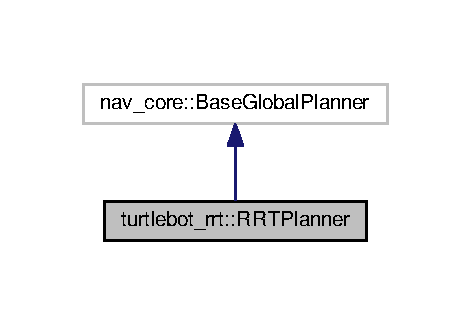
\includegraphics[width=226pt]{classturtlebot__rrt_1_1RRTPlanner__inherit__graph}
\end{center}
\end{figure}


Collaboration diagram for turtlebot\+\_\+rrt\+:\+:R\+R\+T\+Planner\+:
\nopagebreak
\begin{figure}[H]
\begin{center}
\leavevmode
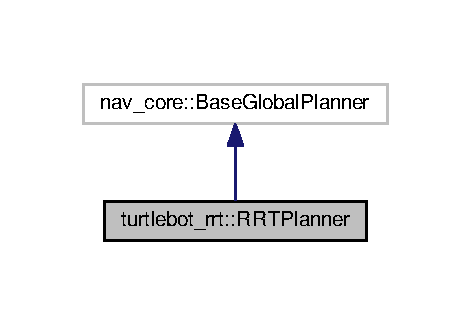
\includegraphics[width=226pt]{classturtlebot__rrt_1_1RRTPlanner__coll__graph}
\end{center}
\end{figure}
\subsection*{Public Member Functions}
\begin{DoxyCompactItemize}
\item 
\hyperlink{classturtlebot__rrt_1_1RRTPlanner_a64bd617e0889067fb6a2514b304939f0}{R\+R\+T\+Planner} ()\hypertarget{classturtlebot__rrt_1_1RRTPlanner_a64bd617e0889067fb6a2514b304939f0}{}\label{classturtlebot__rrt_1_1RRTPlanner_a64bd617e0889067fb6a2514b304939f0}

\begin{DoxyCompactList}\small\item\em Constructor for \hyperlink{classturtlebot__rrt_1_1RRTPlanner}{R\+R\+T\+Planner}. \end{DoxyCompactList}\item 
\hyperlink{classturtlebot__rrt_1_1RRTPlanner_ab6a87e2501b5b750f7c5e6b93bb8fa0a}{R\+R\+T\+Planner} (std\+::string name, costmap\+\_\+2d\+::\+Costmap2\+D\+R\+OS $\ast$costmap\+\_\+ros)
\begin{DoxyCompactList}\small\item\em Constructor for \hyperlink{classturtlebot__rrt_1_1RRTPlanner}{R\+R\+T\+Planner}. \end{DoxyCompactList}\item 
void \hyperlink{classturtlebot__rrt_1_1RRTPlanner_a55b8df1e76bd8daf5411bbaaea058102}{initialize} (std\+::string name, costmap\+\_\+2d\+::\+Costmap2\+D\+R\+OS $\ast$costmap\+\_\+ros)
\begin{DoxyCompactList}\small\item\em Initialize the ros handle. \end{DoxyCompactList}\item 
bool \hyperlink{classturtlebot__rrt_1_1RRTPlanner_a923e270ae622186b06cfbb44fc1b50b0}{make\+Plan} (const geometry\+\_\+msgs\+::\+Pose\+Stamped \&start, const geometry\+\_\+msgs\+::\+Pose\+Stamped \&goal, std\+::vector$<$ geometry\+\_\+msgs\+::\+Pose\+Stamped $>$ \&plan)
\begin{DoxyCompactList}\small\item\em follows the virtual method of the base class \end{DoxyCompactList}\item 
std\+::vector$<$ bool $>$ \hyperlink{classturtlebot__rrt_1_1RRTPlanner_a37827fa1a390fc0014deb4cd487e8079}{get\+Obstacle\+Map} ()
\begin{DoxyCompactList}\small\item\em returns the obstacle map \end{DoxyCompactList}\item 
std\+::vector$<$ \hyperlink{classturtlebot__rrt_1_1Vertex}{turtlebot\+\_\+rrt\+::\+Vertex} $>$ \hyperlink{classturtlebot__rrt_1_1RRTPlanner_a7fa3dc4af8671dea1261f91d995442d9}{get\+Vertex\+Tree} ()\hypertarget{classturtlebot__rrt_1_1RRTPlanner_a7fa3dc4af8671dea1261f91d995442d9}{}\label{classturtlebot__rrt_1_1RRTPlanner_a7fa3dc4af8671dea1261f91d995442d9}

\begin{DoxyCompactList}\small\item\em returns the rrt vertex tree \end{DoxyCompactList}\item 
std\+::pair$<$ float, float $>$ \hyperlink{classturtlebot__rrt_1_1RRTPlanner_a85eeb91e48f93df556e549be8d39a4ad}{Get\+Random\+Point} ()
\begin{DoxyCompactList}\small\item\em Gets a random point in the map space. \end{DoxyCompactList}\item 
int \hyperlink{classturtlebot__rrt_1_1RRTPlanner_a8379a32f6eae2b178b3f76982fa4f9f9}{Get\+Closest\+Vertex} (std\+::pair$<$ float, float $>$ random\+\_\+point)
\begin{DoxyCompactList}\small\item\em Gets the closest vertex to the given point. \end{DoxyCompactList}\item 
void \hyperlink{classturtlebot__rrt_1_1RRTPlanner_ab5be64444ba31b9ddcf2e1b134d0c5f8}{add\+Vertex} (\hyperlink{classturtlebot__rrt_1_1Vertex}{turtlebot\+\_\+rrt\+::\+Vertex} new\+\_\+vertex)
\begin{DoxyCompactList}\small\item\em adds a new vertex to the rrt vertex tree \end{DoxyCompactList}\item 
float \hyperlink{classturtlebot__rrt_1_1RRTPlanner_a5836b6fe15e2d33e753868b0f95f0c3f}{Get\+Distance} (std\+::pair$<$ float, float $>$ start\+\_\+point, std\+::pair$<$ float, float $>$ end\+\_\+point)
\begin{DoxyCompactList}\small\item\em Euclidean distance between two points. \end{DoxyCompactList}\item 
bool \hyperlink{classturtlebot__rrt_1_1RRTPlanner_a21e3230c57b811d41d87439aaad5d052}{Move\+Towards\+Point} (int closest\+\_\+vertex, std\+::pair$<$ float, float $>$ random\+\_\+point)
\begin{DoxyCompactList}\small\item\em Moves from the closest vertex towards the random point  Begins at the closest point and attempts to move step\+\_\+size\+\_\+ towards the random point. Each step along the way at delta\+\_\+ intervals is checked for obstacles. If an obstacle is encountered the function returns false. If it makes it from the closest vertex to step\+\_\+size\+\_\+ towards the random point a new vertex is created and added to vertex\+\_\+list\+\_\+ and the function returns true. \end{DoxyCompactList}\item 
bool \hyperlink{classturtlebot__rrt_1_1RRTPlanner_a86f3447362049feed7251a99d0c2a4a4}{Reached\+Goal} (int new\+\_\+vertex)
\begin{DoxyCompactList}\small\item\em Is vertex within goal\+\_\+radius\+\_\+ of the goal. \end{DoxyCompactList}\item 
std\+::vector$<$ geometry\+\_\+msgs\+::\+Pose\+Stamped $>$ \hyperlink{classturtlebot__rrt_1_1RRTPlanner_a91ceb6a9aa57b6e18df4e74bd95a07b3}{Build\+Plan} (int goal\+\_\+index, const geometry\+\_\+msgs\+::\+Pose\+Stamped \&start, const geometry\+\_\+msgs\+::\+Pose\+Stamped \&goal)
\begin{DoxyCompactList}\small\item\em builds the plan from vertices and returns in Pose\+Stamped \end{DoxyCompactList}\item 
int \hyperlink{classturtlebot__rrt_1_1RRTPlanner_a6e4ef816e70c37f222da73fa40b78b38}{Find\+Path} (const geometry\+\_\+msgs\+::\+Pose\+Stamped \&start, const geometry\+\_\+msgs\+::\+Pose\+Stamped \&goal)
\begin{DoxyCompactList}\small\item\em returns the best path \end{DoxyCompactList}\item 
bool \hyperlink{classturtlebot__rrt_1_1RRTPlanner_a969afbff1661ae9a6738159065f280a0}{Is\+Safe} (std\+::pair$<$ float, float $>$ start\+\_\+point, std\+::pair$<$ float, float $>$ end\+\_\+point)
\begin{DoxyCompactList}\small\item\em Checks if the path is safe between start\+\_\+point and end\+\_\+point. \end{DoxyCompactList}\end{DoxyCompactItemize}


\subsection{Constructor \& Destructor Documentation}
\index{turtlebot\+\_\+rrt\+::\+R\+R\+T\+Planner@{turtlebot\+\_\+rrt\+::\+R\+R\+T\+Planner}!R\+R\+T\+Planner@{R\+R\+T\+Planner}}
\index{R\+R\+T\+Planner@{R\+R\+T\+Planner}!turtlebot\+\_\+rrt\+::\+R\+R\+T\+Planner@{turtlebot\+\_\+rrt\+::\+R\+R\+T\+Planner}}
\subsubsection[{\texorpdfstring{R\+R\+T\+Planner(std\+::string name, costmap\+\_\+2d\+::\+Costmap2\+D\+R\+O\+S $\ast$costmap\+\_\+ros)}{RRTPlanner(std::string name, costmap_2d::Costmap2DROS *costmap_ros)}}]{\setlength{\rightskip}{0pt plus 5cm}turtlebot\+\_\+rrt\+::\+R\+R\+T\+Planner\+::\+R\+R\+T\+Planner (
\begin{DoxyParamCaption}
\item[{std\+::string}]{name, }
\item[{costmap\+\_\+2d\+::\+Costmap2\+D\+R\+OS $\ast$}]{costmap\+\_\+ros}
\end{DoxyParamCaption}
)}\hypertarget{classturtlebot__rrt_1_1RRTPlanner_ab6a87e2501b5b750f7c5e6b93bb8fa0a}{}\label{classturtlebot__rrt_1_1RRTPlanner_ab6a87e2501b5b750f7c5e6b93bb8fa0a}


Constructor for \hyperlink{classturtlebot__rrt_1_1RRTPlanner}{R\+R\+T\+Planner}. 


\begin{DoxyParams}{Parameters}
{\em costmap\+\_\+ros} & cost\+\_\+map ros wrapper \\
\hline
{\em name} & name to associate to the node \\
\hline
\end{DoxyParams}


\subsection{Member Function Documentation}
\index{turtlebot\+\_\+rrt\+::\+R\+R\+T\+Planner@{turtlebot\+\_\+rrt\+::\+R\+R\+T\+Planner}!add\+Vertex@{add\+Vertex}}
\index{add\+Vertex@{add\+Vertex}!turtlebot\+\_\+rrt\+::\+R\+R\+T\+Planner@{turtlebot\+\_\+rrt\+::\+R\+R\+T\+Planner}}
\subsubsection[{\texorpdfstring{add\+Vertex(turtlebot\+\_\+rrt\+::\+Vertex new\+\_\+vertex)}{addVertex(turtlebot_rrt::Vertex new_vertex)}}]{\setlength{\rightskip}{0pt plus 5cm}void turtlebot\+\_\+rrt\+::\+R\+R\+T\+Planner\+::add\+Vertex (
\begin{DoxyParamCaption}
\item[{{\bf turtlebot\+\_\+rrt\+::\+Vertex}}]{new\+\_\+vertex}
\end{DoxyParamCaption}
)\hspace{0.3cm}{\ttfamily [inline]}}\hypertarget{classturtlebot__rrt_1_1RRTPlanner_ab5be64444ba31b9ddcf2e1b134d0c5f8}{}\label{classturtlebot__rrt_1_1RRTPlanner_ab5be64444ba31b9ddcf2e1b134d0c5f8}


adds a new vertex to the rrt vertex tree 


\begin{DoxyParams}{Parameters}
{\em new\+\_\+vertex} & the new vertex to be added \\
\hline
\end{DoxyParams}
\index{turtlebot\+\_\+rrt\+::\+R\+R\+T\+Planner@{turtlebot\+\_\+rrt\+::\+R\+R\+T\+Planner}!Build\+Plan@{Build\+Plan}}
\index{Build\+Plan@{Build\+Plan}!turtlebot\+\_\+rrt\+::\+R\+R\+T\+Planner@{turtlebot\+\_\+rrt\+::\+R\+R\+T\+Planner}}
\subsubsection[{\texorpdfstring{Build\+Plan(int goal\+\_\+index, const geometry\+\_\+msgs\+::\+Pose\+Stamped \&start, const geometry\+\_\+msgs\+::\+Pose\+Stamped \&goal)}{BuildPlan(int goal_index, const geometry_msgs::PoseStamped &start, const geometry_msgs::PoseStamped &goal)}}]{\setlength{\rightskip}{0pt plus 5cm}std\+::vector$<$ geometry\+\_\+msgs\+::\+Pose\+Stamped $>$ turtlebot\+\_\+rrt\+::\+R\+R\+T\+Planner\+::\+Build\+Plan (
\begin{DoxyParamCaption}
\item[{int}]{goal\+\_\+index, }
\item[{const geometry\+\_\+msgs\+::\+Pose\+Stamped \&}]{start, }
\item[{const geometry\+\_\+msgs\+::\+Pose\+Stamped \&}]{goal}
\end{DoxyParamCaption}
)}\hypertarget{classturtlebot__rrt_1_1RRTPlanner_a91ceb6a9aa57b6e18df4e74bd95a07b3}{}\label{classturtlebot__rrt_1_1RRTPlanner_a91ceb6a9aa57b6e18df4e74bd95a07b3}


builds the plan from vertices and returns in Pose\+Stamped 


\begin{DoxyParams}{Parameters}
{\em goal\+\_\+index} & the index of the vertex that has reached the goal \\
\hline
{\em start} & the starting location of the robot as passed to make\+Plan \\
\hline
{\em goal} & the goal location of the robot as passed to make\+Plan \\
\hline
\end{DoxyParams}
\begin{DoxyReturn}{Returns}
a vector of geometry\+\_\+msgs\+:Pose\+Stamped from the start to the goal 
\end{DoxyReturn}
\index{turtlebot\+\_\+rrt\+::\+R\+R\+T\+Planner@{turtlebot\+\_\+rrt\+::\+R\+R\+T\+Planner}!Find\+Path@{Find\+Path}}
\index{Find\+Path@{Find\+Path}!turtlebot\+\_\+rrt\+::\+R\+R\+T\+Planner@{turtlebot\+\_\+rrt\+::\+R\+R\+T\+Planner}}
\subsubsection[{\texorpdfstring{Find\+Path(const geometry\+\_\+msgs\+::\+Pose\+Stamped \&start, const geometry\+\_\+msgs\+::\+Pose\+Stamped \&goal)}{FindPath(const geometry_msgs::PoseStamped &start, const geometry_msgs::PoseStamped &goal)}}]{\setlength{\rightskip}{0pt plus 5cm}int turtlebot\+\_\+rrt\+::\+R\+R\+T\+Planner\+::\+Find\+Path (
\begin{DoxyParamCaption}
\item[{const geometry\+\_\+msgs\+::\+Pose\+Stamped \&}]{start, }
\item[{const geometry\+\_\+msgs\+::\+Pose\+Stamped \&}]{goal}
\end{DoxyParamCaption}
)}\hypertarget{classturtlebot__rrt_1_1RRTPlanner_a6e4ef816e70c37f222da73fa40b78b38}{}\label{classturtlebot__rrt_1_1RRTPlanner_a6e4ef816e70c37f222da73fa40b78b38}


returns the best path 


\begin{DoxyParams}{Parameters}
{\em start} & starting point of robot \\
\hline
{\em goal} & goal point \\
\hline
\end{DoxyParams}
\begin{DoxyReturn}{Returns}
returns the index of the point that reaches the goal 
\end{DoxyReturn}
\index{turtlebot\+\_\+rrt\+::\+R\+R\+T\+Planner@{turtlebot\+\_\+rrt\+::\+R\+R\+T\+Planner}!Get\+Closest\+Vertex@{Get\+Closest\+Vertex}}
\index{Get\+Closest\+Vertex@{Get\+Closest\+Vertex}!turtlebot\+\_\+rrt\+::\+R\+R\+T\+Planner@{turtlebot\+\_\+rrt\+::\+R\+R\+T\+Planner}}
\subsubsection[{\texorpdfstring{Get\+Closest\+Vertex(std\+::pair$<$ float, float $>$ random\+\_\+point)}{GetClosestVertex(std::pair< float, float > random_point)}}]{\setlength{\rightskip}{0pt plus 5cm}int turtlebot\+\_\+rrt\+::\+R\+R\+T\+Planner\+::\+Get\+Closest\+Vertex (
\begin{DoxyParamCaption}
\item[{std\+::pair$<$ float, float $>$}]{random\+\_\+point}
\end{DoxyParamCaption}
)}\hypertarget{classturtlebot__rrt_1_1RRTPlanner_a8379a32f6eae2b178b3f76982fa4f9f9}{}\label{classturtlebot__rrt_1_1RRTPlanner_a8379a32f6eae2b178b3f76982fa4f9f9}


Gets the closest vertex to the given point. 


\begin{DoxyParams}{Parameters}
{\em random\+\_\+point} & A point in the map space \\
\hline
{\em vertex\+\_\+list} & the rrt vertex tree \\
\hline
\end{DoxyParams}
\begin{DoxyReturn}{Returns}
the index of the closest vertex to the given point 
\end{DoxyReturn}
\index{turtlebot\+\_\+rrt\+::\+R\+R\+T\+Planner@{turtlebot\+\_\+rrt\+::\+R\+R\+T\+Planner}!Get\+Distance@{Get\+Distance}}
\index{Get\+Distance@{Get\+Distance}!turtlebot\+\_\+rrt\+::\+R\+R\+T\+Planner@{turtlebot\+\_\+rrt\+::\+R\+R\+T\+Planner}}
\subsubsection[{\texorpdfstring{Get\+Distance(std\+::pair$<$ float, float $>$ start\+\_\+point, std\+::pair$<$ float, float $>$ end\+\_\+point)}{GetDistance(std::pair< float, float > start_point, std::pair< float, float > end_point)}}]{\setlength{\rightskip}{0pt plus 5cm}float turtlebot\+\_\+rrt\+::\+R\+R\+T\+Planner\+::\+Get\+Distance (
\begin{DoxyParamCaption}
\item[{std\+::pair$<$ float, float $>$}]{start\+\_\+point, }
\item[{std\+::pair$<$ float, float $>$}]{end\+\_\+point}
\end{DoxyParamCaption}
)}\hypertarget{classturtlebot__rrt_1_1RRTPlanner_a5836b6fe15e2d33e753868b0f95f0c3f}{}\label{classturtlebot__rrt_1_1RRTPlanner_a5836b6fe15e2d33e753868b0f95f0c3f}


Euclidean distance between two points. 


\begin{DoxyParams}{Parameters}
{\em start\+\_\+point} & starting point \\
\hline
{\em end\+\_\+point} & ending point \\
\hline
\end{DoxyParams}
\begin{DoxyReturn}{Returns}
euclidean distance between the points 
\end{DoxyReturn}
\index{turtlebot\+\_\+rrt\+::\+R\+R\+T\+Planner@{turtlebot\+\_\+rrt\+::\+R\+R\+T\+Planner}!get\+Obstacle\+Map@{get\+Obstacle\+Map}}
\index{get\+Obstacle\+Map@{get\+Obstacle\+Map}!turtlebot\+\_\+rrt\+::\+R\+R\+T\+Planner@{turtlebot\+\_\+rrt\+::\+R\+R\+T\+Planner}}
\subsubsection[{\texorpdfstring{get\+Obstacle\+Map()}{getObstacleMap()}}]{\setlength{\rightskip}{0pt plus 5cm}std\+::vector$<$bool$>$ turtlebot\+\_\+rrt\+::\+R\+R\+T\+Planner\+::get\+Obstacle\+Map (
\begin{DoxyParamCaption}
{}
\end{DoxyParamCaption}
)\hspace{0.3cm}{\ttfamily [inline]}}\hypertarget{classturtlebot__rrt_1_1RRTPlanner_a37827fa1a390fc0014deb4cd487e8079}{}\label{classturtlebot__rrt_1_1RRTPlanner_a37827fa1a390fc0014deb4cd487e8079}


returns the obstacle map 

\begin{DoxyReturn}{Returns}
std\+::vector$<$bool$>$ Unsafe cells are false, safe cells are true 
\end{DoxyReturn}
\index{turtlebot\+\_\+rrt\+::\+R\+R\+T\+Planner@{turtlebot\+\_\+rrt\+::\+R\+R\+T\+Planner}!Get\+Random\+Point@{Get\+Random\+Point}}
\index{Get\+Random\+Point@{Get\+Random\+Point}!turtlebot\+\_\+rrt\+::\+R\+R\+T\+Planner@{turtlebot\+\_\+rrt\+::\+R\+R\+T\+Planner}}
\subsubsection[{\texorpdfstring{Get\+Random\+Point()}{GetRandomPoint()}}]{\setlength{\rightskip}{0pt plus 5cm}std\+::pair$<$ float, float $>$ turtlebot\+\_\+rrt\+::\+R\+R\+T\+Planner\+::\+Get\+Random\+Point (
\begin{DoxyParamCaption}
{}
\end{DoxyParamCaption}
)}\hypertarget{classturtlebot__rrt_1_1RRTPlanner_a85eeb91e48f93df556e549be8d39a4ad}{}\label{classturtlebot__rrt_1_1RRTPlanner_a85eeb91e48f93df556e549be8d39a4ad}


Gets a random point in the map space. 

\begin{DoxyReturn}{Returns}
returns an x,y pair 
\end{DoxyReturn}
\index{turtlebot\+\_\+rrt\+::\+R\+R\+T\+Planner@{turtlebot\+\_\+rrt\+::\+R\+R\+T\+Planner}!initialize@{initialize}}
\index{initialize@{initialize}!turtlebot\+\_\+rrt\+::\+R\+R\+T\+Planner@{turtlebot\+\_\+rrt\+::\+R\+R\+T\+Planner}}
\subsubsection[{\texorpdfstring{initialize(std\+::string name, costmap\+\_\+2d\+::\+Costmap2\+D\+R\+O\+S $\ast$costmap\+\_\+ros)}{initialize(std::string name, costmap_2d::Costmap2DROS *costmap_ros)}}]{\setlength{\rightskip}{0pt plus 5cm}void turtlebot\+\_\+rrt\+::\+R\+R\+T\+Planner\+::initialize (
\begin{DoxyParamCaption}
\item[{std\+::string}]{name, }
\item[{costmap\+\_\+2d\+::\+Costmap2\+D\+R\+OS $\ast$}]{costmap\+\_\+ros}
\end{DoxyParamCaption}
)}\hypertarget{classturtlebot__rrt_1_1RRTPlanner_a55b8df1e76bd8daf5411bbaaea058102}{}\label{classturtlebot__rrt_1_1RRTPlanner_a55b8df1e76bd8daf5411bbaaea058102}


Initialize the ros handle. 

overridden classes from interface nav\+\_\+core\+::\+Base\+Global\+Planner 
\begin{DoxyParams}{Parameters}
{\em name} & R\+OS Node\+Handle name \\
\hline
{\em costmap\+\_\+ros} & cost\+\_\+map ros wrapper \\
\hline
\end{DoxyParams}
\index{turtlebot\+\_\+rrt\+::\+R\+R\+T\+Planner@{turtlebot\+\_\+rrt\+::\+R\+R\+T\+Planner}!Is\+Safe@{Is\+Safe}}
\index{Is\+Safe@{Is\+Safe}!turtlebot\+\_\+rrt\+::\+R\+R\+T\+Planner@{turtlebot\+\_\+rrt\+::\+R\+R\+T\+Planner}}
\subsubsection[{\texorpdfstring{Is\+Safe(std\+::pair$<$ float, float $>$ start\+\_\+point, std\+::pair$<$ float, float $>$ end\+\_\+point)}{IsSafe(std::pair< float, float > start_point, std::pair< float, float > end_point)}}]{\setlength{\rightskip}{0pt plus 5cm}bool turtlebot\+\_\+rrt\+::\+R\+R\+T\+Planner\+::\+Is\+Safe (
\begin{DoxyParamCaption}
\item[{std\+::pair$<$ float, float $>$}]{start\+\_\+point, }
\item[{std\+::pair$<$ float, float $>$}]{end\+\_\+point}
\end{DoxyParamCaption}
)}\hypertarget{classturtlebot__rrt_1_1RRTPlanner_a969afbff1661ae9a6738159065f280a0}{}\label{classturtlebot__rrt_1_1RRTPlanner_a969afbff1661ae9a6738159065f280a0}


Checks if the path is safe between start\+\_\+point and end\+\_\+point. 


\begin{DoxyParams}{Parameters}
{\em start\+\_\+point} & starting point location \\
\hline
{\em end\+\_\+point} & ending point location \\
\hline
\end{DoxyParams}
\begin{DoxyReturn}{Returns}
true if path between points does not intersect obstacles 
\end{DoxyReturn}
\index{turtlebot\+\_\+rrt\+::\+R\+R\+T\+Planner@{turtlebot\+\_\+rrt\+::\+R\+R\+T\+Planner}!make\+Plan@{make\+Plan}}
\index{make\+Plan@{make\+Plan}!turtlebot\+\_\+rrt\+::\+R\+R\+T\+Planner@{turtlebot\+\_\+rrt\+::\+R\+R\+T\+Planner}}
\subsubsection[{\texorpdfstring{make\+Plan(const geometry\+\_\+msgs\+::\+Pose\+Stamped \&start, const geometry\+\_\+msgs\+::\+Pose\+Stamped \&goal, std\+::vector$<$ geometry\+\_\+msgs\+::\+Pose\+Stamped $>$ \&plan)}{makePlan(const geometry_msgs::PoseStamped &start, const geometry_msgs::PoseStamped &goal, std::vector< geometry_msgs::PoseStamped > &plan)}}]{\setlength{\rightskip}{0pt plus 5cm}bool turtlebot\+\_\+rrt\+::\+R\+R\+T\+Planner\+::make\+Plan (
\begin{DoxyParamCaption}
\item[{const geometry\+\_\+msgs\+::\+Pose\+Stamped \&}]{start, }
\item[{const geometry\+\_\+msgs\+::\+Pose\+Stamped \&}]{goal, }
\item[{std\+::vector$<$ geometry\+\_\+msgs\+::\+Pose\+Stamped $>$ \&}]{plan}
\end{DoxyParamCaption}
)}\hypertarget{classturtlebot__rrt_1_1RRTPlanner_a923e270ae622186b06cfbb44fc1b50b0}{}\label{classturtlebot__rrt_1_1RRTPlanner_a923e270ae622186b06cfbb44fc1b50b0}


follows the virtual method of the base class 


\begin{DoxyParams}{Parameters}
{\em start} & start pose \\
\hline
{\em goal} & goal pose \\
\hline
{\em plan} & generated path \\
\hline
\end{DoxyParams}
\begin{DoxyReturn}{Returns}
bool, true 
\end{DoxyReturn}
\index{turtlebot\+\_\+rrt\+::\+R\+R\+T\+Planner@{turtlebot\+\_\+rrt\+::\+R\+R\+T\+Planner}!Move\+Towards\+Point@{Move\+Towards\+Point}}
\index{Move\+Towards\+Point@{Move\+Towards\+Point}!turtlebot\+\_\+rrt\+::\+R\+R\+T\+Planner@{turtlebot\+\_\+rrt\+::\+R\+R\+T\+Planner}}
\subsubsection[{\texorpdfstring{Move\+Towards\+Point(int closest\+\_\+vertex, std\+::pair$<$ float, float $>$ random\+\_\+point)}{MoveTowardsPoint(int closest_vertex, std::pair< float, float > random_point)}}]{\setlength{\rightskip}{0pt plus 5cm}bool turtlebot\+\_\+rrt\+::\+R\+R\+T\+Planner\+::\+Move\+Towards\+Point (
\begin{DoxyParamCaption}
\item[{int}]{closest\+\_\+vertex, }
\item[{std\+::pair$<$ float, float $>$}]{random\+\_\+point}
\end{DoxyParamCaption}
)}\hypertarget{classturtlebot__rrt_1_1RRTPlanner_a21e3230c57b811d41d87439aaad5d052}{}\label{classturtlebot__rrt_1_1RRTPlanner_a21e3230c57b811d41d87439aaad5d052}


Moves from the closest vertex towards the random point  Begins at the closest point and attempts to move step\+\_\+size\+\_\+ towards the random point. Each step along the way at delta\+\_\+ intervals is checked for obstacles. If an obstacle is encountered the function returns false. If it makes it from the closest vertex to step\+\_\+size\+\_\+ towards the random point a new vertex is created and added to vertex\+\_\+list\+\_\+ and the function returns true. 

\begin{DoxyReturn}{Returns}
true if a move was made, false if blocked by obstacle 
\end{DoxyReturn}
\index{turtlebot\+\_\+rrt\+::\+R\+R\+T\+Planner@{turtlebot\+\_\+rrt\+::\+R\+R\+T\+Planner}!Reached\+Goal@{Reached\+Goal}}
\index{Reached\+Goal@{Reached\+Goal}!turtlebot\+\_\+rrt\+::\+R\+R\+T\+Planner@{turtlebot\+\_\+rrt\+::\+R\+R\+T\+Planner}}
\subsubsection[{\texorpdfstring{Reached\+Goal(int new\+\_\+vertex)}{ReachedGoal(int new_vertex)}}]{\setlength{\rightskip}{0pt plus 5cm}bool turtlebot\+\_\+rrt\+::\+R\+R\+T\+Planner\+::\+Reached\+Goal (
\begin{DoxyParamCaption}
\item[{int}]{new\+\_\+vertex}
\end{DoxyParamCaption}
)}\hypertarget{classturtlebot__rrt_1_1RRTPlanner_a86f3447362049feed7251a99d0c2a4a4}{}\label{classturtlebot__rrt_1_1RRTPlanner_a86f3447362049feed7251a99d0c2a4a4}


Is vertex within goal\+\_\+radius\+\_\+ of the goal. 


\begin{DoxyParams}{Parameters}
{\em the} & vertex to be checked \\
\hline
\end{DoxyParams}
\begin{DoxyReturn}{Returns}
true if within goal\+\_\+radius\+\_\+ 
\end{DoxyReturn}


The documentation for this class was generated from the following files\+:\begin{DoxyCompactItemize}
\item 
/home/bob/catkin\+\_\+ws/src/agv\+\_\+navigation/include/turtlebot\+\_\+rrt/turtlebot\+\_\+rrt.\+hpp\item 
/home/bob/catkin\+\_\+ws/src/agv\+\_\+navigation/src/turtlebot\+\_\+rrt.\+cpp\end{DoxyCompactItemize}

\hypertarget{classturtlebot__rrt_1_1Vertex}{}\section{turtlebot\+\_\+rrt\+:\+:Vertex Class Reference}
\label{classturtlebot__rrt_1_1Vertex}\index{turtlebot\+\_\+rrt\+::\+Vertex@{turtlebot\+\_\+rrt\+::\+Vertex}}
\subsection*{Public Member Functions}
\begin{DoxyCompactItemize}
\item 
\hyperlink{classturtlebot__rrt_1_1Vertex_a08a9a7531fe92edd3618661deb182a1c}{Vertex} ()\hypertarget{classturtlebot__rrt_1_1Vertex_a08a9a7531fe92edd3618661deb182a1c}{}\label{classturtlebot__rrt_1_1Vertex_a08a9a7531fe92edd3618661deb182a1c}

\begin{DoxyCompactList}\small\item\em Simple \hyperlink{classturtlebot__rrt_1_1Vertex}{Vertex} constructor. \end{DoxyCompactList}\item 
\hyperlink{classturtlebot__rrt_1_1Vertex_aa613d6a7411e6b4317711d928ab4a9c5}{Vertex} (float x, float y, int index, int parent\+\_\+index)
\begin{DoxyCompactList}\small\item\em the constructor for a \hyperlink{classturtlebot__rrt_1_1Vertex}{Vertex} \end{DoxyCompactList}\item 
\hyperlink{classturtlebot__rrt_1_1Vertex_ab3159441d4b9dff836fa895b8d7f0081}{$\sim$\+Vertex} ()\hypertarget{classturtlebot__rrt_1_1Vertex_ab3159441d4b9dff836fa895b8d7f0081}{}\label{classturtlebot__rrt_1_1Vertex_ab3159441d4b9dff836fa895b8d7f0081}

\begin{DoxyCompactList}\small\item\em destructor \end{DoxyCompactList}\item 
void \hyperlink{classturtlebot__rrt_1_1Vertex_a3eae280de131550a7b69fda426933e24}{set\+\_\+location} (float x, float y)
\begin{DoxyCompactList}\small\item\em sets the location \end{DoxyCompactList}\item 
void \hyperlink{classturtlebot__rrt_1_1Vertex_ada62799b4c6cba1ba5fc812a935c7487}{set\+\_\+index} (int index)
\begin{DoxyCompactList}\small\item\em sets the index of the vertex \end{DoxyCompactList}\item 
void \hyperlink{classturtlebot__rrt_1_1Vertex_a84efb31fdc47e4e2b4283100029db265}{set\+\_\+parent} (int index)
\begin{DoxyCompactList}\small\item\em sets the parent vertex \end{DoxyCompactList}\item 
std\+::pair$<$ float, float $>$ \hyperlink{classturtlebot__rrt_1_1Vertex_aa71422cc4c6d3cc363478beaedf23a88}{get\+\_\+location} ()
\begin{DoxyCompactList}\small\item\em returns the x,y location of the vertex \end{DoxyCompactList}\item 
int \hyperlink{classturtlebot__rrt_1_1Vertex_a63512ad96a03558512b69280329761b8}{get\+\_\+index} ()
\begin{DoxyCompactList}\small\item\em returns the index of the vertex \end{DoxyCompactList}\item 
int \hyperlink{classturtlebot__rrt_1_1Vertex_a41cae85656e4b2e32bee26ba5876b6d1}{get\+\_\+parent} ()
\begin{DoxyCompactList}\small\item\em returns the index of the parent vertex \end{DoxyCompactList}\item 
bool \hyperlink{classturtlebot__rrt_1_1Vertex_a1c743214d3566891fb0c88c60c337a08}{operator==} (const \hyperlink{classturtlebot__rrt_1_1Vertex}{Vertex} \&v)\hypertarget{classturtlebot__rrt_1_1Vertex_a1c743214d3566891fb0c88c60c337a08}{}\label{classturtlebot__rrt_1_1Vertex_a1c743214d3566891fb0c88c60c337a08}

\begin{DoxyCompactList}\small\item\em overload of == operator \end{DoxyCompactList}\item 
bool \hyperlink{classturtlebot__rrt_1_1Vertex_a4bde0da65a589b6afc8f5c50aa6b1b2b}{operator!=} (const \hyperlink{classturtlebot__rrt_1_1Vertex}{Vertex} \&v)\hypertarget{classturtlebot__rrt_1_1Vertex_a4bde0da65a589b6afc8f5c50aa6b1b2b}{}\label{classturtlebot__rrt_1_1Vertex_a4bde0da65a589b6afc8f5c50aa6b1b2b}

\begin{DoxyCompactList}\small\item\em overload of != operator \end{DoxyCompactList}\end{DoxyCompactItemize}


\subsection{Constructor \& Destructor Documentation}
\index{turtlebot\+\_\+rrt\+::\+Vertex@{turtlebot\+\_\+rrt\+::\+Vertex}!Vertex@{Vertex}}
\index{Vertex@{Vertex}!turtlebot\+\_\+rrt\+::\+Vertex@{turtlebot\+\_\+rrt\+::\+Vertex}}
\subsubsection[{\texorpdfstring{Vertex(float x, float y, int index, int parent\+\_\+index)}{Vertex(float x, float y, int index, int parent_index)}}]{\setlength{\rightskip}{0pt plus 5cm}turtlebot\+\_\+rrt\+::\+Vertex\+::\+Vertex (
\begin{DoxyParamCaption}
\item[{float}]{x, }
\item[{float}]{y, }
\item[{int}]{index, }
\item[{int}]{parent\+\_\+index}
\end{DoxyParamCaption}
)}\hypertarget{classturtlebot__rrt_1_1Vertex_aa613d6a7411e6b4317711d928ab4a9c5}{}\label{classturtlebot__rrt_1_1Vertex_aa613d6a7411e6b4317711d928ab4a9c5}


the constructor for a \hyperlink{classturtlebot__rrt_1_1Vertex}{Vertex} 


\begin{DoxyParams}{Parameters}
{\em x} & the x coordinate of the vertex \\
\hline
{\em y} & the y coordinate of the vertex \\
\hline
{\em index} & the index of the vertex \\
\hline
{\em parent\+\_\+index} & the index of the parent vertex \\
\hline
\end{DoxyParams}


\subsection{Member Function Documentation}
\index{turtlebot\+\_\+rrt\+::\+Vertex@{turtlebot\+\_\+rrt\+::\+Vertex}!get\+\_\+index@{get\+\_\+index}}
\index{get\+\_\+index@{get\+\_\+index}!turtlebot\+\_\+rrt\+::\+Vertex@{turtlebot\+\_\+rrt\+::\+Vertex}}
\subsubsection[{\texorpdfstring{get\+\_\+index()}{get_index()}}]{\setlength{\rightskip}{0pt plus 5cm}int turtlebot\+\_\+rrt\+::\+Vertex\+::get\+\_\+index (
\begin{DoxyParamCaption}
{}
\end{DoxyParamCaption}
)}\hypertarget{classturtlebot__rrt_1_1Vertex_a63512ad96a03558512b69280329761b8}{}\label{classturtlebot__rrt_1_1Vertex_a63512ad96a03558512b69280329761b8}


returns the index of the vertex 

\begin{DoxyReturn}{Returns}
index of the vertex 
\end{DoxyReturn}
\index{turtlebot\+\_\+rrt\+::\+Vertex@{turtlebot\+\_\+rrt\+::\+Vertex}!get\+\_\+location@{get\+\_\+location}}
\index{get\+\_\+location@{get\+\_\+location}!turtlebot\+\_\+rrt\+::\+Vertex@{turtlebot\+\_\+rrt\+::\+Vertex}}
\subsubsection[{\texorpdfstring{get\+\_\+location()}{get_location()}}]{\setlength{\rightskip}{0pt plus 5cm}std\+::pair$<$ float, float $>$ turtlebot\+\_\+rrt\+::\+Vertex\+::get\+\_\+location (
\begin{DoxyParamCaption}
{}
\end{DoxyParamCaption}
)}\hypertarget{classturtlebot__rrt_1_1Vertex_aa71422cc4c6d3cc363478beaedf23a88}{}\label{classturtlebot__rrt_1_1Vertex_aa71422cc4c6d3cc363478beaedf23a88}


returns the x,y location of the vertex 

\begin{DoxyReturn}{Returns}
returns std\+::pair$<$x,y$>$ 
\end{DoxyReturn}
\index{turtlebot\+\_\+rrt\+::\+Vertex@{turtlebot\+\_\+rrt\+::\+Vertex}!get\+\_\+parent@{get\+\_\+parent}}
\index{get\+\_\+parent@{get\+\_\+parent}!turtlebot\+\_\+rrt\+::\+Vertex@{turtlebot\+\_\+rrt\+::\+Vertex}}
\subsubsection[{\texorpdfstring{get\+\_\+parent()}{get_parent()}}]{\setlength{\rightskip}{0pt plus 5cm}int turtlebot\+\_\+rrt\+::\+Vertex\+::get\+\_\+parent (
\begin{DoxyParamCaption}
{}
\end{DoxyParamCaption}
)}\hypertarget{classturtlebot__rrt_1_1Vertex_a41cae85656e4b2e32bee26ba5876b6d1}{}\label{classturtlebot__rrt_1_1Vertex_a41cae85656e4b2e32bee26ba5876b6d1}


returns the index of the parent vertex 

\begin{DoxyReturn}{Returns}
returns the index of the parent 
\end{DoxyReturn}
\index{turtlebot\+\_\+rrt\+::\+Vertex@{turtlebot\+\_\+rrt\+::\+Vertex}!set\+\_\+index@{set\+\_\+index}}
\index{set\+\_\+index@{set\+\_\+index}!turtlebot\+\_\+rrt\+::\+Vertex@{turtlebot\+\_\+rrt\+::\+Vertex}}
\subsubsection[{\texorpdfstring{set\+\_\+index(int index)}{set_index(int index)}}]{\setlength{\rightskip}{0pt plus 5cm}void turtlebot\+\_\+rrt\+::\+Vertex\+::set\+\_\+index (
\begin{DoxyParamCaption}
\item[{int}]{index}
\end{DoxyParamCaption}
)}\hypertarget{classturtlebot__rrt_1_1Vertex_ada62799b4c6cba1ba5fc812a935c7487}{}\label{classturtlebot__rrt_1_1Vertex_ada62799b4c6cba1ba5fc812a935c7487}


sets the index of the vertex 


\begin{DoxyParams}{Parameters}
{\em index} & index of the vertex \\
\hline
\end{DoxyParams}
\index{turtlebot\+\_\+rrt\+::\+Vertex@{turtlebot\+\_\+rrt\+::\+Vertex}!set\+\_\+location@{set\+\_\+location}}
\index{set\+\_\+location@{set\+\_\+location}!turtlebot\+\_\+rrt\+::\+Vertex@{turtlebot\+\_\+rrt\+::\+Vertex}}
\subsubsection[{\texorpdfstring{set\+\_\+location(float x, float y)}{set_location(float x, float y)}}]{\setlength{\rightskip}{0pt plus 5cm}void turtlebot\+\_\+rrt\+::\+Vertex\+::set\+\_\+location (
\begin{DoxyParamCaption}
\item[{float}]{x, }
\item[{float}]{y}
\end{DoxyParamCaption}
)}\hypertarget{classturtlebot__rrt_1_1Vertex_a3eae280de131550a7b69fda426933e24}{}\label{classturtlebot__rrt_1_1Vertex_a3eae280de131550a7b69fda426933e24}


sets the location 


\begin{DoxyParams}{Parameters}
{\em x} & x location of vertex \\
\hline
{\em y} & y location of vertex \\
\hline
\end{DoxyParams}
\index{turtlebot\+\_\+rrt\+::\+Vertex@{turtlebot\+\_\+rrt\+::\+Vertex}!set\+\_\+parent@{set\+\_\+parent}}
\index{set\+\_\+parent@{set\+\_\+parent}!turtlebot\+\_\+rrt\+::\+Vertex@{turtlebot\+\_\+rrt\+::\+Vertex}}
\subsubsection[{\texorpdfstring{set\+\_\+parent(int index)}{set_parent(int index)}}]{\setlength{\rightskip}{0pt plus 5cm}void turtlebot\+\_\+rrt\+::\+Vertex\+::set\+\_\+parent (
\begin{DoxyParamCaption}
\item[{int}]{index}
\end{DoxyParamCaption}
)}\hypertarget{classturtlebot__rrt_1_1Vertex_a84efb31fdc47e4e2b4283100029db265}{}\label{classturtlebot__rrt_1_1Vertex_a84efb31fdc47e4e2b4283100029db265}


sets the parent vertex 


\begin{DoxyParams}{Parameters}
{\em parent\+\_\+index} & index of the parent vertex \\
\hline
\end{DoxyParams}


The documentation for this class was generated from the following files\+:\begin{DoxyCompactItemize}
\item 
/home/bob/catkin\+\_\+ws/src/agv\+\_\+navigation/include/turtlebot\+\_\+rrt/vertex.\+hpp\item 
/home/bob/catkin\+\_\+ws/src/agv\+\_\+navigation/src/\hyperlink{vertex_8cpp}{vertex.\+cpp}\end{DoxyCompactItemize}

\chapter{File Documentation}
\hypertarget{vertex_8cpp}{}\section{/home/bob/catkin\+\_\+ws/src/agv\+\_\+navigation/src/vertex.cpp File Reference}
\label{vertex_8cpp}\index{/home/bob/catkin\+\_\+ws/src/agv\+\_\+navigation/src/vertex.\+cpp@{/home/bob/catkin\+\_\+ws/src/agv\+\_\+navigation/src/vertex.\+cpp}}
{\ttfamily \#include \char`\"{}turtlebot\+\_\+rrt/vertex.\+hpp\char`\"{}}\\*
Include dependency graph for vertex.\+cpp\+:
\nopagebreak
\begin{figure}[H]
\begin{center}
\leavevmode
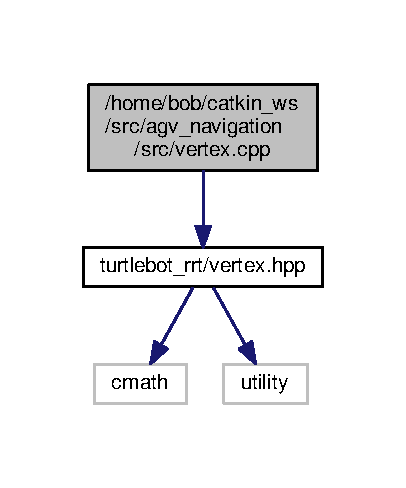
\includegraphics[width=195pt]{vertex_8cpp__incl}
\end{center}
\end{figure}
\subsection*{Namespaces}
\begin{DoxyCompactItemize}
\item 
 \hyperlink{namespaceturtlebot__rrt}{turtlebot\+\_\+rrt}
\end{DoxyCompactItemize}


\subsection{Detailed Description}
\begin{DoxyAuthor}{Author}
Bhargav Dandamudi and Mayank Pathak 
\end{DoxyAuthor}
\begin{DoxyVersion}{Version}
1 
\end{DoxyVersion}
\begin{DoxyDate}{Date}
2018-\/12-\/16 
\end{DoxyDate}

%--- End generated contents ---

% Index
\backmatter
\newpage
\phantomsection
\clearemptydoublepage
\addcontentsline{toc}{chapter}{Index}
\printindex

\end{document}
